\documentclass[a4paper]{scrreprt}

%% Language and font encodings
\usepackage[german]{babel}
\setcounter{secnumdepth}{3} 
\setcounter{tocdepth}{3} 
\usepackage[utf8x]{inputenc}
\usepackage[T1]{fontenc}
\usepackage{courier}
\usepackage{colortbl} 

%% Sets page size and margins
\usepackage[a4paper,top=3cm,bottom=2cm,left=3cm,right=3cm,marginparwidth=1.75cm]{geometry}

%% Useful packages
\usepackage{amsmath}
\usepackage{graphicx}
\usepackage[colorinlistoftodos]{todonotes}
\usepackage[colorlinks=true, allcolors=blue, breaklinks = true]{hyperref}
\usepackage{tocstyle}
\usetocstyle{standard}
\settocfeature{raggedhook}{\raggedright}
\usepackage{longtable}
\usepackage{scrhack}
\usepackage{graphicx}
\usepackage{float}
\graphicspath{ {images/} }

\begin{document}	
	\begin{flushright}
		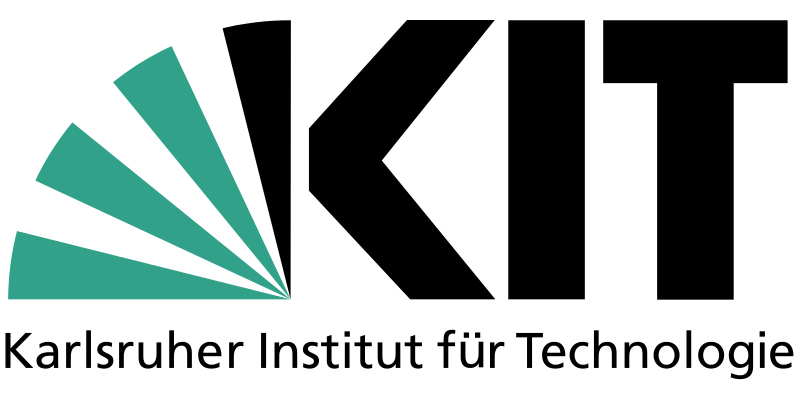
\includegraphics[scale = 0.2]{kit-logo.png}\\[0.5cm]
	\end{flushright}
	\vspace*{2cm}
	
	\begin{center}
		\large Praxis der Softwareentwicklung
		\vspace*{1.5cm}
		
		\textbf{\huge Fridget}
		\vspace*{1cm}
		
		\textbf{\Large Qualitätssicherung Testbericht}
		\vspace*{2cm}
		
		Yunjia Chen, Jasmin Jat, Min Hye Park, Alina Shah, Lisa Wang
		\vspace*{1cm}
		
		\today
		\vspace*{2.5cm}
		
		Betreuung: Erik Burger, Sandro Koch\\[0.5cm]
		IPD\\[0.5cm]
		
		Karlsruher Institut für Technologie
		
	\end{center}

	\thispagestyle{empty}
	
	\tableofcontents
	
	\chapter{Einleitung}
	
	
	\chapter{Gefundene Bugs und deren Behebung}
	Folgende Bugs wurden gefunden:
	\begin{flushleft}
		\begin{longtable}{|p{.32\textwidth}|p{.32\textwidth}|p{.32\textwidth}|}
		\hline
		\textbf{Fehlersymptom} & \textbf{Fehlergrund} & \textbf{Fehlerbehebung} \\
		\hline
		\end{longtable}
	\end{flushleft}	
	
	\chapter{Unit Tests}
	\section{Client}
	\subsection{Activity}
	\subsubsection{public class LoginActivityTest}
	\textbf{Beschreibung}\\
	\textit{Diese Klasse testet das erfolgreiche Builden der LoginActivity.}\\
	\\	
	\textbf{Methoden}
	\begin{itemize}
		
		\item\texttt{{public void setUp() throws Exception}}
		
		\textit{Diese Methode setzt die ActivityTestRule zur LoginActivity auf null.}
		
		\item\texttt{{public void TestLaunch()}}
		
		\textit{Diese Methode testet das Builden der View zur LoginActivity.}
		
		\item\texttt{{public void tearDown()}}
		
		\textit{Diese Methode setzt die ActivityTestRule zur LoginActivity wieder auf null.}
		
		
	\end{itemize}
	\subsubsection{public class StartActivityTest}
	\textbf{Beschreibung}\\
	\textit{Diese Klasse testet das erfolgreiche Builden der StartActivity.}\\
	\\	
	\textbf{Methoden}
	\begin{itemize}
		
		\item\texttt{{public void setUp() throws Exception}}
		
		\textit{Diese Methode setzt die ActivityTestRule zur StartActivity auf null.}
		
		\item\texttt{{public void TestLaunch()}}
		
		\textit{Diese Methode testet das Builden der View zur StartActivity.}
		
		\item\texttt{{public void tearDown()}}
		
		\textit{Diese Methode setzt die ActivityTestRule zur StartActivity wieder auf null.}
		
		
	\end{itemize}
	\subsubsection{public class HomeActivityTest}
	\textbf{Beschreibung}\\
	\textit{Diese Klasse testet das erfolgreiche Builden der HomeActivity.}\\
	\\	
	\textbf{Methoden}
	\begin{itemize}
		
		\item\texttt{{public void setUp() throws Exception}}
		
		\textit{Diese Methode setzt die ActivityTestRule zur HomeActivity auf null.}
		
		\item\texttt{{public void TestLaunch()}}
		
		\textit{Diese Methode testet das Builden der View zur HomeActivity.}
		
		\item\texttt{{public void tearDown()}}
		
		\textit{Diese Methode setzt die ActivityTestRule zur HomeActivity wieder auf null.}
		
		
	\end{itemize}
	\subsubsection{public class CreateFlatshareActivityTest}
	\textbf{Beschreibung}\\
	\textit{Diese Klasse testet das erfolgreiche Builden der CreateFlatshareActivity.}\\
	\\	
	\textbf{Methoden}
	\begin{itemize}
		
		\item\texttt{{public void setUp() throws Exception}}
		
		\textit{Diese Methode setzt die ActivityTestRule zur CreateFlatshareActivity auf null.}
		
		\item\texttt{{public void TestLaunch()}}
		
		\textit{Diese Methode testet das Builden der View zur CreateFlatshareActivity.}
		
		\item\texttt{{public void tearDown()}}
		
		\textit{Diese Methode setzt die ActivityTestRule zur CreateFlatshareActivity wieder auf null.}
		
		
	\end{itemize}
	\subsubsection{public class CreateTextCoolNoteActivityTest}
	\textbf{Beschreibung}\\
	\textit{Diese Klasse testet das erfolgreiche Builden der CreateTextCoolNoteActivity.}\\
	\\	
	\textbf{Methoden}
	\begin{itemize}
		
		\item\texttt{{public void setUp() throws Exception}}
		
		\textit{Diese Methode setzt die ActivityTestRule zur CreateTextCoolNoteActivity auf null.}
		
		\item\texttt{{public void TestLaunch()}}
		
		\textit{Diese Methode testet das Builden der View zur CreateTextCoolNoteActivity.}
		
		\item\texttt{{public void tearDown()}}
		
		\textit{Diese Methode setzt die ActivityTestRule zur CreateTextCoolNoteActivity wieder auf null.}
		
		
	\end{itemize}
	\subsubsection{public class EditTextFrozenNoteActivityTest}
	\textbf{Beschreibung}\\
	\textit{Diese Klasse testet das erfolgreiche Builden der EditTextFrozenNoteActivity.}\\
	\\	
	\textbf{Methoden}
	\begin{itemize}
		
		\item\texttt{{public void setUp() throws Exception}}
		
		\textit{Diese Methode setzt die ActivityTestRule zur EditTextFrozenNoteActivity auf null.}
		
		\item\texttt{{public void TestLaunch()}}
		
		\textit{Diese Methode testet das Builden der View zur EditTextFrozenNoteActivity.}
		
		\item\texttt{{public void tearDown()}}
		
		\textit{Diese Methode setzt die ActivityTestRule zur EditTextFrozenNoteActivity wieder auf null.}
		
		
	\end{itemize}
	\subsubsection{public class EnterAcccessCodeActivityTest}
	\textbf{Beschreibung}\\
	\textit{Diese Klasse testet das erfolgreiche Builden der EnterAccessCodeActivity.}\\
	\\	
	\textbf{Methoden}
	\begin{itemize}
		
		\item\texttt{{public void setUp() throws Exception}}
		
		\textit{Diese Methode setzt die ActivityTestRule zur EnterAccessCodeActivity auf null.}
		
		\item\texttt{{public void TestLaunch()}}
		
		\textit{Diese Methode testet das Builden der View zur EnterAccessCodeActivity.}
		
		\item\texttt{{public void tearDown()}}
		
		\textit{Diese Methode setzt die ActivityTestRule zur EnterAccessCodeActivity wieder auf null.}
		
		
	\end{itemize}
	\subsubsection{public class FullTextFrozenNoteActivityTest}
	\textbf{Beschreibung}\\
	\textit{Diese Klasse testet das erfolgreiche Builden der FullTextFrozenNoteActivity.}\\
	\\	
	\textbf{Methoden}
	\begin{itemize}
		
		\item\texttt{{public void setUp() throws Exception}}
		
		\textit{Diese Methode setzt die ActivityTestRule zur FullTextFrozenNoteActivity auf null.}
		
		\item\texttt{{public void TestLaunch()}}
		
		\textit{Diese Methode testet das Builden der View zur FullTextFrozenNoteActivity.}
		
		\item\texttt{{public void tearDown()}}
		
		\textit{Diese Methode setzt die ActivityTestRule zur FullTextFrozenNoteActivity wieder auf null.}
		
		
	\end{itemize}
	
	\subsection{Viewmodel}
	\subsection{Services}
	\subsubsection{\texttt{public class AccessCodeServiceTest}}
	\textbf{Beschreibung}\\
	\textit{Diese Klasse testet die Requests des Access-Code-Services.}\\
	\\	
	\textbf{Methoden}
	\begin{itemize}

		\item\texttt{{public void setUp() throws Exception}}
		
		\textit{Diese Methode baut die MockRetrofit-Instanz.}
		
		\item\texttt{{public void testGenerateAccesscode() throws Exception}}
		
		\textit{Diese Methode testet das Request zum Generieren eines Zugangscodes.}
		
		
	\end{itemize}
	\subsubsection{\texttt{public class CoolNoteServiceTest}}
	\textbf{Beschreibung}\\
	\textit{Diese Klasse testet die Requests des Cool-Note-Services.}\\
	\\
	\textbf{Methoden}
	\begin{itemize}
		
		\item\texttt{{public void setUp() throws Exception}}
		
		\textit{Diese Methode baut die MockRetrofit-Instanz.}
		
		\item\texttt{{public void testCreateCoolNote() throws IOException}}
		
		\textit{Diese Methode testet das Request zum Erstellen einer Cool Note.}
		
		\item\texttt{{public void testGetAllCoolNotes() throws IOException}}
		
		\textit{Diese Methode testet das Request zum Getten aller Cool Note.}
		
		\item\texttt{{public void testGetCoolNote() throws IOException}}
		
		\textit{Diese Methode testet das Request zum Gettern einer bestimmten Cool Note.}
		
		\item\texttt{{public void testGetCoolNote\_WithIncorrectId() throws IOException}}
		
		\textit{Diese Methode testet das Request zum Getten einer bestimmten Cool Note, wenn eine inkorrekte Cool-Note-Id übergeben wird.}
		
		\item\texttt{{public void testDeleteCoolNote() throws IOException}}
		
		\textit{Diese Methode testet das Request zum Löschen einer Cool Note.}	
		
	\end{itemize}
	\subsubsection{\texttt{public class DeviceServiceTest}}
	\textbf{Beschreibung}\\
	\textit{Diese Klasse testet die Requests des Device-Services.}\\
	\\
	\textbf{Methoden}
	\begin{itemize}
	
		\item\texttt{{public void setUp() throws Exception}}
	
	\textit{Diese Methode baut die MockRetrofit-Instanz.}
	
	\item\texttt{{public void testSendDevice() throws Exception}}
	
	\textit{Diese Methode testet das Request zum Senden eines Devices.}
	
	\end{itemize}
	
	\subsubsection{\texttt{public class FlatshareTestService}}
	\textbf{Beschreibung}\\
	\textit{Diese Klasse testet die Requests des Flatshare-Services.}\\
	\\
	\textbf{Methoden}
	\begin{itemize}
		
		
		\item\texttt{{public void setUp() throws Exception}}
		
		\textit{Diese Methode baut die MockRetrofit-Instanz.}
		
		\item\texttt{{public void testCreateFlatshare() throws Exception}}
		
		\textit{Diese Methode testet das Request zum Erstellen einer WG.}
		
		\item\texttt{{public void testGetFlatshare() throws Exception}}
		
		\textit{Diese Methode testet das Request zum Getten einer WG.}
		
	\end{itemize}
	\subsubsection{\texttt{public class FrozenNozeServiceTest}}
	\textbf{Beschreibung}\\
	\textit{Diese Klasse testet die Requests des Frozen-Note-Services.}\\
	\\
	\textbf{Methoden}
	\begin{itemize}
		
		
		\item\texttt{{public void setUp() throws Exception}}
		
		\textit{Diese Methode baut die MockRetrofit-Instanz.}
		
		\item\texttt{{public void testGetAllFrozenNotes() throws Exception}}
		
		\textit{Diese Methode testet das Request zum Getten aller Frozen Notes.}
		
		\item\texttt{{public void testGetFrozenNote() throws Exception}}
		
		\textit{Diese Methode testet das Request zum Getten einer bestimmten Frozen Note.}
		
		\item\texttt{{public void testUpdateFrozenNote() throws Exception}}
		
		\textit{Diese Methode testet das Request zum Updaten einer Frozen Note.}
		
	\end{itemize}
	\subsubsection{\texttt{public class MembershipServiceTest}}
	\textbf{Beschreibung}\\
	\textit{Diese Klasse testet die Requests des Membership-Services.}\\
	\\
	\textbf{Methoden}
	\begin{itemize}
		
		
		\item\texttt{{public void setUp() throws Exception}}
		
		\textit{Diese Methode baut die MockRetrofit-Instanz.}
		
		\item\texttt{{public void testGetMemberlist() throws Exception}}
		
		\textit{Diese Methode testet das Request zum Getten der Mitgliederliste.}
		
		\item\texttt{{public void testGetMember() throws Exception}}
		
		\textit{Diese Methode testet das Request zum Getten eines bestimmten Mitglieds.}
		
		\item\texttt{{public void testCreateMembership() throws Exception}}
		
		\textit{Diese Methode testet das Request zum Erstellen einer Mitgliedschaft.}
		
		\item\texttt{{public void testDeleteMember() throws Exception}}
		
		\textit{Diese Methode testet das Request zum Löschen eines Mitglieds.}
		
	\end{itemize}
	\subsubsection{\texttt{public class ReadConfirmationServiceTest}}
	\textbf{Beschreibung}\\
	\textit{Diese Klasse testet die Requests des Read-Confirmation-Services.}\\
	\\
	\textbf{Methoden}
	\begin{itemize}
		
		
		\item\texttt{{public void setUp() throws Exception}}
		
		\textit{Diese Methode baut die MockRetrofit-Instanz.}
		
		\item\texttt{{public void testGetReaders() throws Exception}}
		
		\textit{Diese Methode testet das Request zum Getten der Leserliste einer Cool Note.}
		
		\item\texttt{{public void testCreateReadStatus() throws Exception}}
		
		\textit{Diese Methode testet das Request zum Erstellen einer Lesebestätigung.}
		
		\item\texttt{{public void testDeleteReadStatus() throws Exception}}
		
		\textit{Diese Methode testet das Request zum Löschen einer Lesebestätigung.}
		
	\end{itemize}

	\subsubsection{\texttt{public class UserServiceTest}}
	\textbf{Beschreibung}\\
	\textit{Diese Klasse testet die Requests des User-Services.}\\
	\\
	\textbf{Methoden}
	\begin{itemize}
				
		\item\texttt{{public void setUp() throws Exception}}
		
		\textit{Diese Methode baut die MockRetrofit-Instanz.}
		
		\item\texttt{{public void testSendIdToken() throws Exception}}
		
		\textit{Diese Methode testet das Request zum Senden eines Id-Tokens.}
		
	\end{itemize}
	\section{Server}
	
	\chapter{Espresso-Tests}
	\section{Testszenarien}
	
	\chapter{Nutzerstudie}
	

\end{document}
